\graphicspath{{chapter_introduction/}}
\chapter{Introduction}

The landscape of computer vision has shifted dramatically over the
past decade. Prior to this, general purpose solutions to difficult
problems had low success rates on unconstrained images. This is
especially true for the primary focus of this thesis: 3D face
reconstruction. This chapter begins by giving an introduction to the
problem of 3D face reconstruction. We attempt to justify the need for
research in this area by highlighting many of the important
applications, as well as the limitations of existing
work. Additionally, this chapter attempts to explain where our own
work on this problem fits into the area of 3D face
reconstruction. Finally, we give an overview of the structure of this
thesis.

\section{Problem}

3D face reconstruction is the process of estimating the 3D geometry of
a person's face, but what exactly do we even mean by geometry?
Fundamentally, this geometry is a set of 3D vertices, connected by
edges, which together defines a 3D surface. This is more generally
referred to as a mesh. This mesh should capture the shape, expression
and pose of the face. In a perfect world, it should also capture finer
details, such as facial hair, eye brows, eye lashes, wrinkles, spots,
blemishes and anything else we as humans can see on a person's
face. Ideally, it should also capture facial accessories, such as
glasses and jewellery.

Well, even with the laser precision of commercial 3D scanners,
satisfying all of these desires is currently impossible. Despite this,
3D scanners are the go to solution when it comes to obtaining a high
resolution facial mesh. However, the use of such equipment comes with
many limitations. Perhaps worst of all is that the person being
scanned has to sit very still while the scan is being performed,
surrounded by some large and intimidating machine. In fact, haven't we
been here before? This all sounds very similar to photography in the
early 1800's. Mercury vapour aside - ``Sir! Stand still, please! There
is at least five more minutes until our photo has exposed!''

Many applications of 3D face reconstruction cannot tolerate these
constraints. Such examples span a wide range of areas. The more
obvious being personalisation of computer games, or trying on
accessories online, such as glasses. However, this area has many other
applications, such as facial expression analysis for measuring
emotional arousal, where 3D face reconstruction can be a useful tool
in psychological studies. Facial performance transfer is another
potential application of this area of work and is widely used in
creative industries, such as the development of computer games and
animated films where typically a large number facial point markers
have to be attached to the actor's face. Additionally, standing
perfectly still could certainly have a negative impact on the actor's
performance. There is also the potential for medical applications,
such as simulating the result of reconstructive surgery after an
accident.

Due to the nature of these applications, there is a clear demand for
reliability under unconstrained environments, which regularly cannot
be catered to by 3D scanning. As such, there are a variety of
approaches which attempt to perform 3D face reconstruction under more
typical settings. The inputs to these methods vary widely, from sets
of images in predefined poses and video, to reconstruction from a
single unconstrained image. Some of the difficulties which all 3D face
reconstructions would \textit{like} to be able to address are
displayed in Figure~\ref{fig:faceproblems}, and discussed in detail
the next few paragraphs.

\begin{figure}
  \begin{tabular}{cccc}
    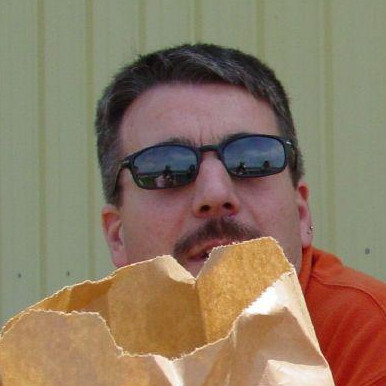
\includegraphics[width=0.22\linewidth]{img/afw/occlusion.jpg} &
    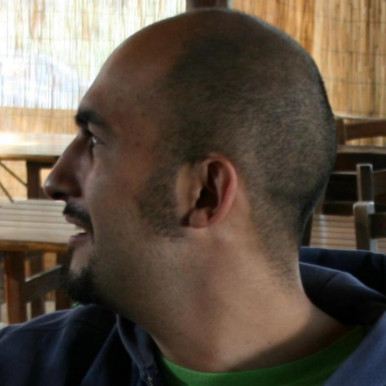
\includegraphics[width=0.22\linewidth]{img/afw/pose.jpg} &
    
\includegraphics[width=0.22\linewidth]{img/afw/illumination.jpg} &
    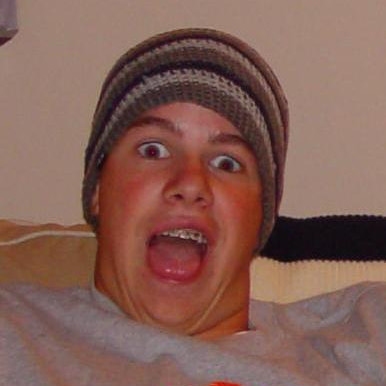
\includegraphics[width=0.22\linewidth]{img/afw/expression.jpg} \\
    Occlusion & Large Pose & Illumination & Expression
  \end{tabular}
  \caption[Visual examples of challenging images]{Some visual examples
    of common problems which 3D Face Reconstruction methods have to be
    able to tolerate, taken from the AFW dataset~\cite{zhu2012face}.}
  \label{fig:faceproblems}
\end{figure}


\paragraph{Occlusion.} In computer vision, occlusion refers to the
visual obstruction of an object. In the case of faces, this could be
due to any number of reasons, from nose scratching to accessory
wearing and beyond. As humans, we can look past this occlusion. Faces
do not suddenly stop being faces just because there's a hand in the
way. We can also make assumptions about what the shape or appearance
of a face might be based on the information available with a high
level of confidence. Unfortunately, this is much harder for a
computer. We have to encode this information some how, and tie pieces
together with knowledge, such as how faces are generally symmetric. An
approach which deals with this problem quite well is to use a 3D
Morphable Model (3DMM), which we'll discuss in much more detail later
in this chapter.

\paragraph{Large Pose} refers to any facial pose which defers too much
from a frontal face, that is, a face which is looking directly at the
camera. For many methods this is between $45^\circ - 90^\circ$, at
which point a large portion of the face is self occluded. Many methods
attempt to work around this problem by using multiple images from
different views. This is referred to as multiview 3D face
reconstruction and has its own set of problems which are discussed
later in this section, other approaches are model based, and are
therefore able to make a reliable assumption about the self occluded
part of the face.

\paragraph{Illumination} can cause issues for many methods. For some
methods, a perfectly illuminated face without any shadows is
optimal. For other methods, such as those based on a
Shape-from-Shading (SfS) approaches, having no shadows at all is
equally as big a problem.

\paragraph{Facial Expression.} Some facial expressions are more
challenging than others, a neutral expression typically being the
easiest to model and often the most prevalent in facial scan
datasets. Take smiling for instance, smiling result in large
deformation of the 3D geometry around the mouth, but also to the sides
of the nose and around the eyes. The extent of this deformation varies
largely from person to person, making many facial expressions
challenging and the relationship between areas of the face under
different expressions difficult to model.

\paragraph{Detail} is difficult for two main reasons. First, an
approach which is capable of encoding a high level of detail is
required. This is often challenging with model fitting based
approaches because the inputs need to be constrained to a small number
of principal components which vary aspects such as shape, pose and
rotation. This constraint usually leads to post-processing steps to
extract the detail, which can destroy correspondence between vertices
usually present in a parametric model, as well as pose and scale
information. Second, there needs to be some way to distinguish between
what is actually \textit{detail}, such as wrinkles and spots which
affect 3D shape versus what is noise, makeup (potentially tattoos),
dirt or anything else affecting only textural information.

\paragraph{Lab Conditions vs. In-the-Wild.} Due to the difficulties
involved with using 3D scanning equipment, discussed earlier, facial
scan datasets are always collected under lab conditions. This
typically limits the amount of variation available across many
aspects, for example lighting and illumination and background
scenery. 3D face reconstruction methods which are then trained on such
data may struggle to transfer their knowledge to what are known as
``In-the-Wild'' images. Such images are very diverse compared to what
may be available under constrained lab conditions.

\paragraph{Single Image vs. Multiview or Video.} Methods capable of
using or requiring multiple views or video often have a lot more
information available to them. Parts of the face which are typically
self occluded under the single image setting may be available to the
method if multiple images are available. However, taking multiple
images of fixed pose and expression is a problem in its own right, and
it is therefore preferable use only a single image without having a
detrimental effect on reconstruction performance.

Our approach to 3D face reconstruction has proven resilient to many of
the aforementioned challenges. We demonstrate good performance on
occluded faces, show only a small reduction in performance for large
poses and difficult facial expressions, work across challenging
illumination on rendered datasets, and work on \textit{in-the-wild}
images and use only a single image. In the case of detail, we
demonstrate that our approach is capable of estimating the fine
details in Chapter~\ref{chapter:human}, in which we demonstrate our
method also working on human body reconstruction with high levels of
detail.

\section{Where do we fit in?}

There are a number of approaches to 3D face reconstruction. Each
general approach has its own set of advantages and disadvantages. The
aim of this section is to give a brief overview of the general
approaches to this problem. By doing so, we hope to show where and how
our own work fits in, along with why we feel this is important.

% 3D Morphable Models
\paragraph{3D Morphable Models (3DMM)} are perhaps the most popular
approach to estimating facial 3D geometry. These methods use a vector
of parameters for a pre-computed face
model~\cite{jourabloo2016large,huber2016multiresolution,zhu2016face,liu2016joint},
which varies the shape, expression, pose and optionally textural
information. We discuss 3DMM in more detail in
Chapter~\ref{chapter:literature}. These methods are increasingly using
Convolutional Neural Networks as a means to regress the parameters,
and in general, work very reliably on \textit{normal} faces. However,
3DMM based approaches gradually perform worse as factors such as pose
and expression increase. We show in
Section~\ref{chapter:face:sec:ablation} that our method has a very
uniform and low error over all expressions, with only a small increase
in error on large poses (such as around 80 degrees). Another
disadvantage of 3DMM based approaches is that the 3DMM must be
generated - this requires finding the dense correspondence between all
vertices of all samples, which also becomes difficult as pose and
expression changes. Finally, since these methods are model based, they
are unable to directly produce finer details, such as wrinkles. In an
extension to our own work, we show in Chapter~\ref{chapter:human}
(where we perform 3D reconstruction of humans), that our method is
able to directly regress fine details in clothing.

\paragraph{Multiview and Photogrammetry} based methods require
multiple images from many different angles in order to estimate the 3D
geometry of a face (or other
object)~\cite{dou2018multi,dai2018coarse,Piotraschke_2016_CVPR,mayo20093d}. The
primary drawback of such methods is, of course, that multiple images
are not always available, especially under the aforementioned
environmental constraints associated with 3D face
reconstruction. While the final 3D reconstruction from such methods
can be of very high resolution and detailed, finding corresponding
features between each image is both memory and CPU intensive. Our own
method uses only a single RGB image, without any additional depth data
- from this single image, we regress the full 3D facial geometry.

\paragraph{Shape-from-Shading (SfS)} methods attempt to recover the 3D
geometry by analysing the shading and reflectance of a face relative
to a \textit{albedo} (mean) face. Similarly to 3DMM based methods, SfS
methods often rely on a 3D model, inheriting many of the same
problems, such as finding a dense
correspondence~\cite{suwajanakorn2014total,jiang20183d}. Additionally,
many of these methods also require more than one image, which means
SfS methods often also inherit the problems associated with multiview
methods. Finally, more so than other methods, SfS methods struggle
with lighting - over or under illuminated faces may produce poor
results when compared to other methods. Our approach to 3D face
reconstruction works under almost all kinds of lighting, and we show
this on a challenging synthetic dataset.

\paragraph{Depth Estimation} is arguable more popular among problems
such as room reconstruction, however, there are several methods which
attempt to reconstruct the frontal part of the facial 3D geometry
using this technique~\cite{sun2011depth,sun2013depth}. It would be
fair to claim that these methods have declined in popularity. The
biggest flaw of depth estimation based approaches is that only the
visible parts can be reconstructed, unless other methods are employed
afterwards (such as 3DMM, again, inheriting many of the aforementioned
problems). While also working from a single image, our method is able
to hallucinate the non-visible parts of the face, including, to a
certain extent, those which have been self occluded without having to
handle this cases on an individual basis.

Given the numerous applications of such a technology and the
significant disadvantages of the preexisting methods, we feel there is
a profound requirement for something more robust to the challenges in
this area. In this thesis we approach the problem using a single
image, and propose a new non-parametric approach to 3D face
reconstruction which attempts to account for as many of these
challenges as possible.

\section{Contributions}

The contributions of this thesis can be summarised as follows:

\begin{itemize}
\item %
  We propose an alternative representation for the 3D geometry which,
  unlike $X, Y, Z$ vertices, can be directly regressed using a
  Convolutional Neural Network (CNN). Our method is non-parametric and
  does not use a shape model. This offers the advantage of being able
  to regress detail without further post processing steps.

\item % 3D face reconstruction
  We present a deeply learnt method for 3D face reconstruction, which
  can be trained directly in an end-to-end fashion. Our method
  reconstructs the full 3D facial structure, including parts which are
  occluded. We also show that our method works from just a single
  images without requiring accurate alignment or establishing a dense
  correspondence between all training samples.  This allows us to
  bypass the construction (during training) and fitting (during
  inference) of a 3D Morphable Model (3DMM).  We refer to this method
  as the \textbf{Volumetric Regression Network (VRN)}.

\item We show how a related task of facial landmark localisation can
  be incorporated into our method (also in an end-to-end fashion) to
  improve the reconstruction quality, particularly on faces of large
  pose and expression.

\item We evaluate our method on both constrained and heavily
  unconstrained images from the web, demonstrating that our method
  \textbf{outperforms all prior work} on single image 3D face
  reconstruction by a large margin.

\item We show that our method works on other deformable objects, such
  as in the task of \textbf{human body reconstruction}, and that
  provided high quality training data is available, our method is able
  to both reconstruct difficult human poses and \textbf{fine details
    such as wrinkles} in clothing.

\item We release our code for 3D face reconstruction under the MIT
  license, enabling our method to be used for both commercial and
  personal purposes. In addition, we have provided a free online
  service for automatic generation of 3D reconstructions from an
  uploaded image.
\end{itemize}

\section{Outline}

In \textbf{Chapter~\ref{chapter:background}}, an introduction to the
background material is provided, discussing volumetric representations
and algorithms, such as voxelisation, surface extraction and some of
the difficulties associated with volumetric representations.

\textbf{Chapter~\ref{chapter:literature}} gives an overview of related
literature, starting with face alignment, which is often a
prerequisite to 3D face reconstruction methods. Continuing on, a
discussion of the various existing 3D face reconstruction is
given. The remainder of this chapter gives an overview of human pose
estimation and human body reconstruction.

\textbf{Chapter~\ref{chapter:face}} is the primary focus of this
thesis. This chapter describes our approach to 3D face reconstruction,
which includes details about the datasets used, the volumetric
representation and the (small) amount of error it introduces, along
with our approach and network architectures. This chapter also
describes the numerous experiments carried out on the various
datasets, comparisons with other methods, and ablation studies on
pose, expression and influence of parameters used for
guidance. Finally, we explore some of the architectural options
available for this method, which result in performance degradation or
boosts.

An extension to our work on 3D face reconstruction is described in
\textbf{Chapter~\ref{chapter:human}}, in which we show how our method
can be applied to on another category of deformable objects: the full
human body. We carry out experiments on two datasets, showing that our
approach can handle both difficult poses and finer details.

Our first work, focusing on landmark guided semantic part segmentation
of the human face is described in
\textbf{Chapter~\ref{chapter:seg}}. It is important to mention here
that this thesis does not focus on semantic segmentation, but this
work \textit{heavily} influenced our approach to the problem of 3D
reconstruction, since our method shifts the 3D reconstruction problem
into a volumetric segmentation problem.

Finally, we conclude with a reflection and discussion of our work,
what impact it may have had and the numerous areas worthy of attention
as future work, in \textbf{Chapter~\ref{chapter:conclusion}}.

\section{Publications}

Several publications came as a result of the work leading up to this
thesis:

\begin{itemize}
\item Jackson, A.S., Valstar, M. and Tzimiropoulos, G., 2016,
  October. A CNN cascade for landmark guided semantic part
  segmentation. In European Conference on Computer Vision (Workshops)
  (pp. 143-155). Springer, Cham.

\item Jackson, A.S., Bulat, A., Argyriou, V. and Tzimiropoulos, G.,
  2017, October. Large pose 3D face reconstruction from a single
  image via direct volumetric CNN regression. In Computer Vision
  (ICCV), 2017 IEEE International Conference on
  (pp. 1031-1039). IEEE.

\item Jackson, A.S., Manafas, C., \& Tzimiropoulos, G., 2018 3D
  Human Body Reconstruction from a Single Image via Volumetric
  Regression. In European Conference on Computer Vision (Workshops).
\end{itemize}

%%% Local Variables:
%%% TeX-master: "../thesis"
%%% End:
